% Chapter 4
\newenvironment{my_desc}
{\begin{description}
  \setlength{\itemsep}{0cm}
  \setlength{\parskip}{0cm}}
{\end{description}}

\chapter{Smart Email Requirements and Design} % Main chapter title

\label{Chapter4} % For referencing the chapter elsewhere, use \ref{Chapter4} 

\lhead{Chapter 4. \emph{Smart Email Requirements and Design}} % This is for the header on each page - perhaps a shortened title

\section{Introduction}
In chapter \ref{Chapter3}, the features of the smart email classifier were presented.

In this chapter, software requirements specification and software design description 
are explained in sections \ref{sec:4_SRS} and \ref{sec:4_SDD} respectively. The chapter is
concluded in section \ref{sec:conclusion_4}.

\section{Software Requirements Specification} % Main chapter title
\label{sec:4_SRS}
%==============================================================================
\subsection{Overview}
In this section, an overview about the software requirements specification
is shown, such as, project objective, assumptions, limitations, open items
and risks.

\subsubsection{Project Objective}
The business objective of this project is building a web service that provides
automatic email categorization into user-defined folders based on machine 
learning and data mining classification techniques.

%==============================================================================

\subsubsection{Assumptions}
Some assumptions must be generally made in order to write a brief definition 
of the application. Some assumptions are technical, while others are business natured.  Assumptions 
critical to the success of this project are listed below:
\begin{my_itemize}
  \item each user will have his own trained classification model based on the user supplied training data;
  \item a web service will be implemented to provide email classification support for different email 
	providers (for example: Google, Hotmail, Yahoo);
  \item english language will be supported by default;
  \item the servers providing the web service have to provide sufficient 
	processing power for achieving reasonable response time;
  \item email classification will be based on the email subject and content. 
	Other features can be used as well, such as the email sender and recepient(s). 
	However, email attachments will not be considered as a classification feature for the email.
\end{my_itemize}

%==============================================================================
\subsubsection{Limitations}
Some limitations are assumptions on the extent of feature scope. Others are restrictions on resources 
or methods for achieving the objectives. The limitations of this project are listed below:

\begin{my_itemize}
  \item sufficient number of emails is needed for each email label to achieve 
	a reasonable classification accuracy;
  \item emails with size less than a specified threshold won't be classified with
  high accuracy.
\end{my_itemize}

%==============================================================================
\subsubsection{Open items and Risks}
During the analysis of the project and in the process of writing this document, 
some issues remain open.
\begin{my_itemize}
  \item Multi-label classification.
  \item Arabic support.
  \item Securing the communication between the client and the classification web service.
  \item Improving classification accuracy.
  \item Specifications for the web server providing the web service.
\end{my_itemize}


%==============================================================================
\subsection{Proposed Workflow}
%==============================================================================
\subsubsection{Overview}
This section includes a concise description of the features and operation of the 
proposed solution. The context and workflow of the proposed solution are defined in subsequent sections.

Features:
\begin{my_itemize}
  \item Register users with the classification web service and build a classification model for each user.
  \item Automatically classify emails into user-defined folders.
  \item Monitor email accounts to be classify new incoming emails automatically.
  \item Provide classification related statistics for the user.
  \item Accept user feedback on classified emails.
  \item Re-train the classifier based on user feedback.
\end{my_itemize}

%==============================================================================
\subsubsection{Context Diagram}
The Context Diagram in figure 4.1 illustrates the modules, business processes, ...etc that feed 
or interact with this proposed application.
\begin{figure}[H]
  \centering
  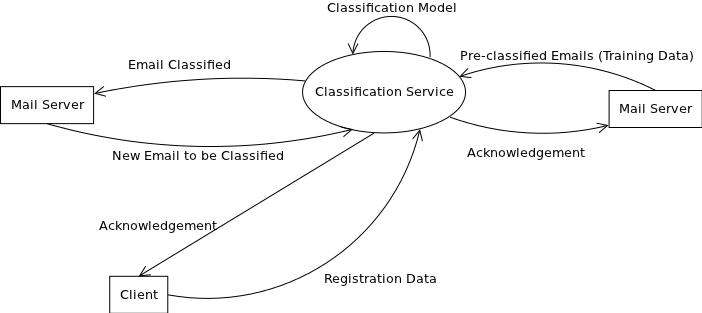
\includegraphics[width=13cm]{context_diagram.png}
  \caption[The Context Diagram illustrates the modules, business processes, ...etc that feed 
or interact with this proposed application.] {The Context Diagram illustrates the modules, business processes, ...etc that feed 
or interact with this proposed application.}
\end{figure}


%==============================================================================
\subsubsection{High Level Workflow}
The workflow required to complete the primary objectives of the proposed 
application is described below. The workflow is business-centered, and 
includes ``decision forks'' for decisions the business user, or application, 
must make to achieve the objective. The workflow omits application faults or exceptions. 
Individual tasks in the workflow are described.

\begin{my_enumerate}
  \item Workflow/Process Map 
	
\begin{figure}[H]
  \centering
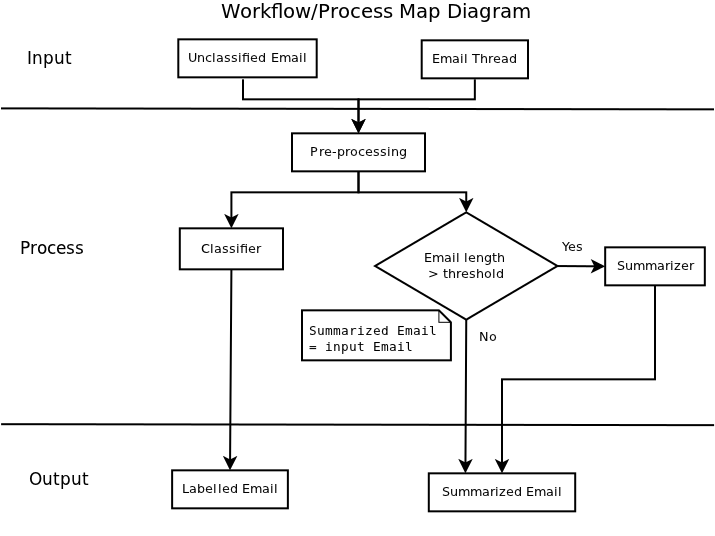
\includegraphics[width=13cm]{workflow_process_map.png}
  \caption[Workflow Process] {Workflow Process}
\end{figure}

  \item Workflow Description
  \begin{my_itemize}
    \item Incoming Emails are preprocessed.
    \item Classification module uses the user model to classify the email into a specific label.
    \item The result is returned by the web service.
  \end{my_itemize}
\end{my_enumerate}

%==============================================================================
\subsubsection{User stories}
Breaking up the system components to user stories with estimated time (in terms
of man-days = 4 hours) to finish the story is very good practice.
\\

\begin{tabular}{|p{3cm}|p{10cm}|}
\hline
\cellcolor[gray]{0.9} Story Id & \#1 \\ \hline
\cellcolor[gray]{0.9} User Story & Authentication \\ \hline
\cellcolor[gray]{0.9} Priority & Low \\ \hline
\cellcolor[gray]{0.9} Description & 
      As a \textbf{User}, I can \textbf{authenticate the application}. \\ \hline
\cellcolor[gray]{0.9} Estimated time & 1 man-day \\ \hline
\cellcolor[gray]{0.9} Notes & 
      Authentication is done with email username and password. \\ \hline
\end{tabular}

\begin{tabular}{|p{3cm}|p{10cm}|}
\hline
\cellcolor[gray]{0.9} Story Id & \#2 \\ \hline
\cellcolor[gray]{0.9} User Story & Deauthentication \\ \hline
\cellcolor[gray]{0.9} Priority & Low \\ \hline
\cellcolor[gray]{0.9} Description & 
	As a \textbf{User}, I can \textbf{deauthenticate the application}. \\ \hline
\cellcolor[gray]{0.9} Estimated time & 1 man-day \\ \hline
\cellcolor[gray]{0.9} Notes & 
	Authentication is done with email username and password. \\ \hline
\end{tabular}

\begin{tabular}{|p{3cm}|p{10cm}|}
\hline
\cellcolor[gray]{0.9} Story Id & \#3 \\ \hline
\cellcolor[gray]{0.9} User Story & Label suggestion \\ \hline
\cellcolor[gray]{0.9} Priority & Medium\\ \hline
\cellcolor[gray]{0.9} Description & 
	As a \textbf{User}, I can \textbf{give feedback for the chosen/suggested labels} to
	\textbf{enhance the classification accuracy}. \\ \hline
\cellcolor[gray]{0.9} Estimated time & 5 man-days\\ \hline
\cellcolor[gray]{0.9} Notes & 
	Build browser extension to support suggestions in gmail. \\ \hline
\end{tabular}

\begin{tabular}{|p{3cm}|p{10cm}|}
\hline
\cellcolor[gray]{0.9} Story Id & \#4 \\ \hline
\cellcolor[gray]{0.9} User Story & Data pre-processing \\ \hline
\cellcolor[gray]{0.9} Priority & High\\ \hline
\cellcolor[gray]{0.9} Description & 
	As a \textbf{System}, I can \textbf{preprocess the dataset} to
	\textbf{make it ready for the classification}. \\ \hline
\cellcolor[gray]{0.9} Estimated time & 4 man-days\\ \hline
\cellcolor[gray]{0.9} Notes & 
	Preprocessing includes stemming, checking email length/language,
	removing stop words and identifying the features. \\ \hline
\end{tabular}

\begin{tabular}{|p{3cm}|p{10cm}|}
\hline
\cellcolor[gray]{0.9} Story Id & \#5 \\ \hline
\cellcolor[gray]{0.9} User Story & Email Classification \\ \hline
\cellcolor[gray]{0.9} Priority & High\\ \hline
\cellcolor[gray]{0.9} Description & 
	As a \textbf{System}, I can \textbf{make online classification to
	an incoming email}. \\ \hline
\cellcolor[gray]{0.9} Estimated time & 20 man-days\\ \hline
\cellcolor[gray]{0.9} Notes & 
	More than one algorithm will be implemented to choose the one with 
	the best accuracy. \\ \hline
\end{tabular}

\begin{tabular}{|p{3cm}|p{10cm}|}
\hline
\cellcolor[gray]{0.9} Story Id & \#6 \\ \hline
\cellcolor[gray]{0.9} User Story & User Classification Model \\ \hline
\cellcolor[gray]{0.9} Priority & High\\ \hline
\cellcolor[gray]{0.9} Description & 
	As a \textbf{System}, I can \textbf{build a user classification 
	model from the training data}. \\ \hline
\cellcolor[gray]{0.9} Estimated time & 5 man-days\\ \hline
\cellcolor[gray]{0.9} Notes & 
	It will start after user authentication, and can be applied 
	from time to time to enhance the user model. \\ \hline
\end{tabular}

\begin{tabular}{|p{3cm}|p{10cm}|}
\hline
\cellcolor[gray]{0.9} Story Id & \#7 \\ \hline
\cellcolor[gray]{0.9} User Story & Classification Accuracy test \\ \hline
\cellcolor[gray]{0.9} Priority & Medium \\ \hline
\cellcolor[gray]{0.9} Description & 
	As an \textbf{Admin}, I can \textbf{test the accuracy of the 
	classification algorithm at runtime}. \\ \hline
\cellcolor[gray]{0.9} Estimated time & 2 man-days\\ \hline
\cellcolor[gray]{0.9} Notes & 
	The admin can view the accuracy of the used classification algorithm. \\ \hline
\end{tabular}

%==============================================================================
\newpage
\subsection{Business Requirements}

This section identifies, enumerates and explores the business requirements that must 
be met by the application. Business requirements include capturing the types of users, 
the basic inputs and outputs, the system's dependencies, and the tasks the system should 
accomplish. It is important to confirm that Task Requirements include all the tasks 
required to meet the business objectives.

%==============================================================================
\subsubsection{Users}
All applications have users and most of them have several users of different types. This 
section identifies, at a high level, the types of users of the system.

\begin{my_enumerate}
  \item Application User: requests emails classification.
  \item Admin: tunes classification algorithms and observes the results.
\end{my_enumerate}

%==============================================================================
\subsubsection{Inputs/Outputs}
This section identifies and describes the inputs to and outputs from the new 
application. In this section, all electronic inputs and outputs 
are captured. Human inputs are omitted from this section.

\begin{my_enumerate}
  \item Inputs:
  \begin{my_itemize}
    \item unclassified Emails;
    \item classified Emails (training data);
  \end{my_itemize}
  \item Outputs:
  \begin{my_itemize}
    \item classified emails;
    \item classification model.
  \end{my_itemize}
\end{my_enumerate}


%==============================================================================
\subsubsection{Dependencies}
Human inputs are also categorized as dependencies.
\begin{my_enumerate}
  \item IMAP service in the email provider.
  \item Registration data.
  \item Number of emails in each user-defined label (affects classification model)
\end{my_enumerate}


%==============================================================================
\subsubsection{Security Requirements}
This section documents, at a high level, the basic security requirements of the 
application. For example, does the system require the user to login?  Should the 
user’s identity be authenticated on just this system, or against a central authority?  
Are there any special or unusual security requirements, like fingerprint scanning?

\begin{my_enumerate}
  \item The system requires every user to login with a unique identity (email).
  \item User Data (email) should be transmitted through a secure connection.
  \item Administrators shouldn’t have access to user data (email).
\end{my_enumerate}



%==============================================================================
\subsubsection{Performance Requirements}
Performance Requirements for the application are defined at a high level below. 
If there are specific requirements for specific features to perform at a quantifiable 
level, they too are listed below. These requirements will be developed in more detail when 
the Requirements Specification is written, in a later phase.

\begin{my_enumerate}
  \item Classification web service should respond within a reasonable time.
  \item Initial training phase should finish within a reasonable time.
  \item The system will achieve high uptime.
\end{my_enumerate}


%==============================================================================
\subsubsection{Data Migration}
Data Migration describes the data that needs to be moved from an older or external 
system to the new system, in order for it to operate at launch. Migration also includes 
data that must be transferred from the new system to another external system. 
Any data migration requirements are listed below.

\begin{my_enumerate}
  \item Users' classified emails for training phase as pre-classified emails are needed to build users' models.
  \item Users' feedback on the results of the classification.
\end{my_enumerate}

%==============================================================================

\section{Software Design Description (SDD)}
\label{sec:4_SDD}
%------------------------------------------------------------------------------

\subsection{Purpose}
This section shows how the Smart Email software system will be 
structured to satisfy the requirements identified in the software
requirements specification section. It is a translation of 
requirements into a description of the software structure, software components, 
interfaces, and data necessary for the implementation phase.

\subsection{Scope}
Smart email will provide automated email classification for email clients. 
This section describes how the system will be divided into modules and 
the design details for each module.


\subsection{Decomposition description}
There are three primary stages to the design development which consists of phase 1 
(Classification Web Service Module), phase 2 (Email Monitoring Web Service Module),
and phase 3 (Web Browser Extension).

The classification module can be divided into three layers. The data layer will be 
responsible for retrieving emails from file systems or using IMAP protocol. The 
second layer is the preprocessing and email filtering layer. This layer is 
responsible for filtering emails and extracting classification features from the 
email. The third and last layer will be responsible for classifying emails and 
testing the classifier performance.

The detailed design for each entity is illustrated in the detailed class 
diagram at the end of this section.

\subsubsection{System decomposition}
The system is divided into main modules as follows:
\begin{my_itemize}
  \item classification web service;
  \item email monitoring web service;
  \item web browser extension.
\end{my_itemize}
Each of these modules will be described in details in the upcoming subsections.

\paragraph{Classification Web Service}

Classification web service provides an API for the email classification service.
\begin{my_itemize}
	\item user registeration: A user can register with the service with one or more email accounts. The service trains using the user's email dataset, builds a classification model and stores it in a database.
	
	\item unregisteration: The user can remove himself from the service.

	\item classification request: The user can send a classification request for any email. The system will retrieve the user model, classify the email and send the classification result back to the user.

	\item feedback: In case the system classifies an email to an incorrect folder, the user can send feedback to the system with the correct folder. The system will use this feedback to improve future classification.

\end{my_itemize}

\paragraph{Email Monitoring Web Service} 

Email Monitoring Web Service is a web service implemented in RubyOnRails \cite{ROR} framework which integrates 
with a classification web service for classification of emails. The web service monitors 
users emails and sends every new email to the classification service through a REST API \cite{REST}
which returns a response with the email label, the web service then applies the label to the user’s email.

\begin{itemize}
 \item MVC illustration for the Email Monitoring module
 \begin{figure}[H]
   \centering
   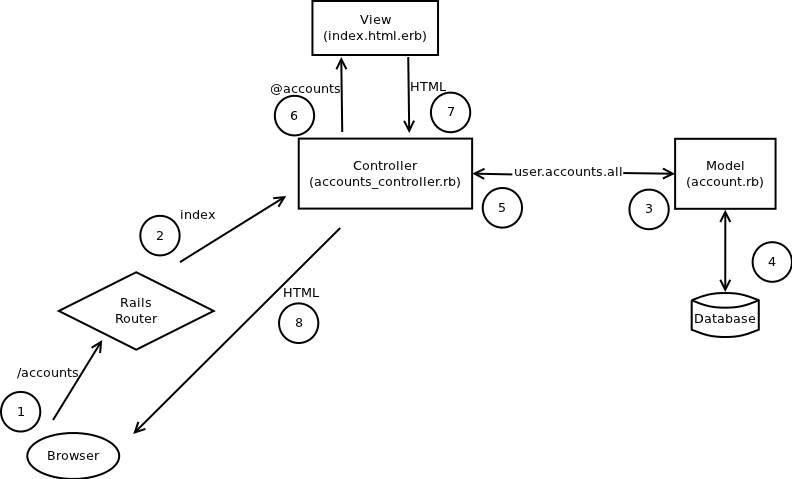
\includegraphics[width=12cm]{account_example.png}
   \caption[Example for MVC in action handling a user request to view his 
   accounts]{Example for MVC in action handling a user request to view his accounts}
 \end{figure}

 \item Features
 \begin{itemize}
    \item Users registration.
    \item Adding more than one email account.
    \item Continuous monitoring of emails accounts for new emails.
 \end{itemize}
 
 \item Future Work
  \begin{itemize}
    \item Providing statistics about the classification process.
    \item Support email providers other than Gmail: Yahoo, Hotmail, ...etc.
    \item Classifying users into active and non-active ones based on their 
    email account activity to decrease the load and increase the performance 
    of the monitoring process.
    \item Improving performance and security.
  \end{itemize}
\end{itemize}

\paragraph{Web Browser Extension}
Web Browser Extension is a client side browser extension that injects a 
``Classify Me'' button when the user open the email which is an additional 
UI component injected into the user's email web interface. 


\begin{itemize}
 \item Features
 \begin{itemize}
    \item Users registration.
    \item Sending a classification requests to the classification web service.
    \item Check the status of the user's training phase at the classification 
    web service.
    \item Sending feedback to the classification web service when the user
    applies labels manually to an email to re-train the model.
 \end{itemize}
 \item Future Work
  \begin{itemize}
    \item Providing statistics about the classification process.
    \item Support other web browsers other than Chrome extension: Firefox, 
    Safari, ...etc.
    \item Improving performance and security.
  \end{itemize}
\end{itemize}

\subsubsection{Data decomposition}
The data layer is responsible for retrieving emails either from the file system or using 
the IMAP protocol. The Enron dataset \cite{ENRON} will be used as the data source for training and 
testing the email classifier.

\begin{my_desc}
  \item[Data access object] this class is used to provide an abstract way to retrieve emails.
  \item[IMAP Data access object] it is responsible for retrieving emails using the IMAP protocol,
  and it inherits the Data access object class.
  \item[File system data access object] it is responsible for retrieving emails from the file
  system, and it inherits the Data access object class.
\end{my_desc}


%==============================================================================
\subsection{Interface description}
The interface description provides everything designers, programmers and 
testers need to know how to correctly use the functions provided by the system 
entities. This description includes the details of external and internal 
interfaces not provided in the software requirements specification.

\subsubsection{Module interface}
\paragraph{Classification Web Service API}
%\begin{itemize}
    \begin{itemize} %TODO: edit this to the new REST API
      \item register(username,password) adds user to database and starts training phase
      \item remove(username,password) removes user information from database.
      \item status(username) returns current status of training phase.
      \item classify(emailContent) returns the best category for this email.
      \item classify(email\_imap\_id) returns the best category for this email.
      \item feedback(email\_content,correct\_label) retrains the model using the new instance.
    \end{itemize}
%\end{itemize}

%-------
\newpage
\paragraph{Email Monitoring Web Service API}
\begin{itemize}
	\item API for user registration
	\begin{itemize}
		\item Basic URL: http://smart-email.herokuapp.com/
		\item Endpoint: /users
		\item Request type: POST
		\item Parameters: username, password
		\item Response: Success/Error on creating the new user
	\end{itemize}

	\item API for email account registration
	\begin{itemize}
		\item Basic URL: http://smart-email.herokuapp.com/
		\item Endpoint: /accounts
		\item Request type: POST
		\item Parameters: username, password
		\item Response: Success/Error on creating the new user
	\end{itemize}
\end{itemize}

%==============================================================================
\newpage
\subsubsection{Detailed design}
\paragraph{Classification module detailed design}
.\\
\begin{figure}[H]
  \centering
  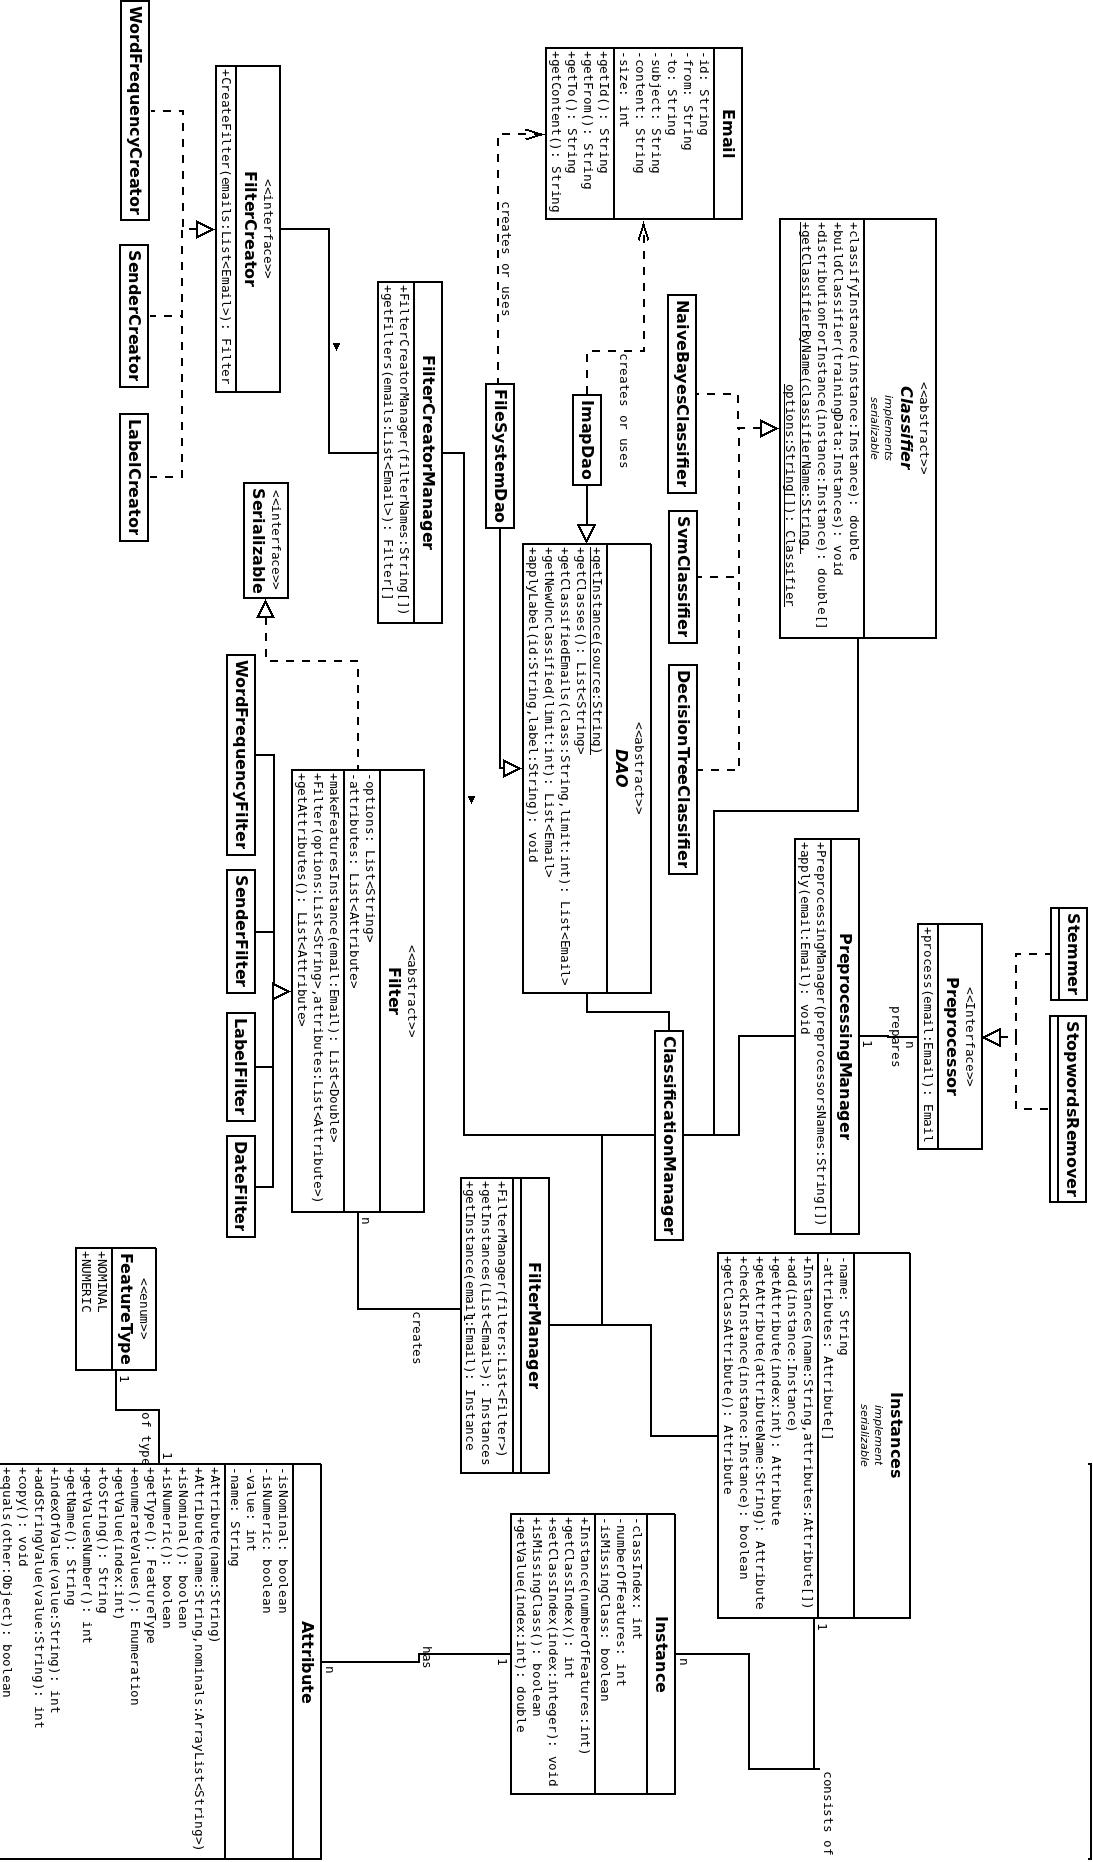
\includegraphics[width=12cm]{design.jpeg}
  \caption[Detailed Design] {Detailed Design}
\end{figure}



\paragraph{Email Monitoring Web service module detailed design}
.\\
\begin{figure}[H]
  \centering
  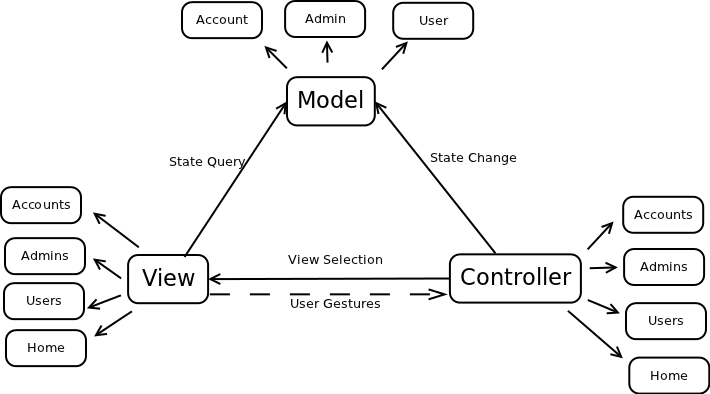
\includegraphics[width=15cm]{mvc2.png}
  \caption[Smart Email MVC Design]{Smart Email MVC Design}
\end{figure}


\section{Conclusion}
\label{sec:conclusion_4}
In this chapter, the software requirements specification and software design
description were discussed. While in the next chapter, Environment and 
Development tools will be discussed.
